\documentclass[../report.tex]{subfiles}

\begin{document}
Trong phần này, chúng ta sẽ xem xét giá trị của các 
tập mờ trong một hệ động học mờ $(F_k^1[0, 1], z_f)$. \\
\subsection{Các ví dụ hệ động học mờ}

\noindent \textbf{Ví dụ 2}: Tính toán nguyên lý mở rộng Zadeh bởi $f$ được 
cho bởi tam giá $(0, 0), (1/4, 9/10), (1, 0)$
và tập mờ $A$ được cho bởi $(0, 0), (3/4, 1), (1, 0)$ như trong 
hình \ref{fig:2}.
\begin{figure}[H]
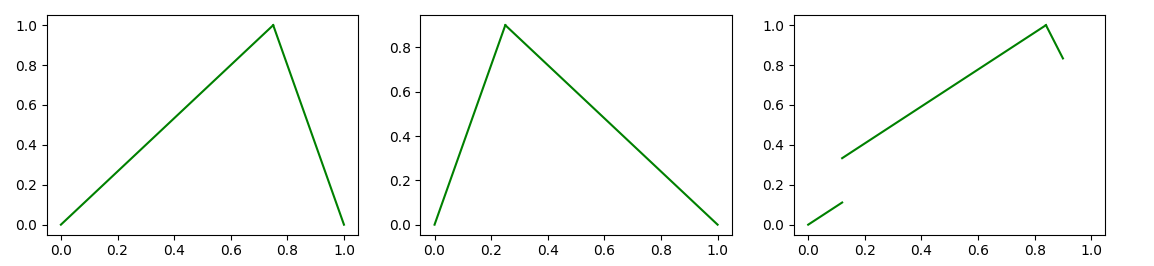
\includegraphics[width=\textwidth]{figures/example2.png}
\caption{Đồ thị của tập mờ $A$, hàm $f$ và $z_f^2(A)$}
\label{fig:2}
\end{figure}

Từ hình trên ta có thể thấy, cho dù với những đồ thị rất đơn giản cho 
các hàm tuyến tính liên tục $f$ và $A$, nguyên lý mở rộng Zadeh 
có thể sinh ra những tập mờ không liên tục, như trong ví dụ trên
$z_f^2(A)$ là không liên tục. Trong hình \ref{fig:3}, 20 giá trị đầu tiên
của quỹ đạo mờ được thể hiện trên đồ thị 3 chiều. 

\begin{figure}[H]
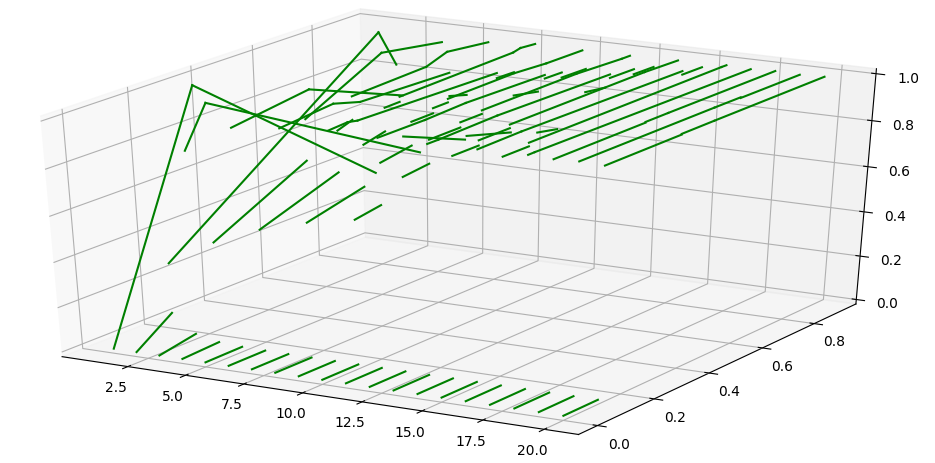
\includegraphics[width=\textwidth]{figures/example2_3d.png}
\caption{20 giá trị đầu tiên của quỹ đạo}
\label{fig:3}
\end{figure}

\noindent \textbf{Ví dụ 3}: Trong ví dụ này ta xem xét đến ánh 
xạ piecewise linear liên tục f và tập mờ piecewise linear 
liên tục A được mô tả trong hình \ref{fig:4}. 30 vòng lặp đầu 
tiên được biểu thị trong hình \ref{fig:5} và hình \ref{fig:6}.
Ta có thể thấy, quỹ đạo của chất điểm trở nên tuần hoàn theo 
thời gian. 

\begin{figure}[H]
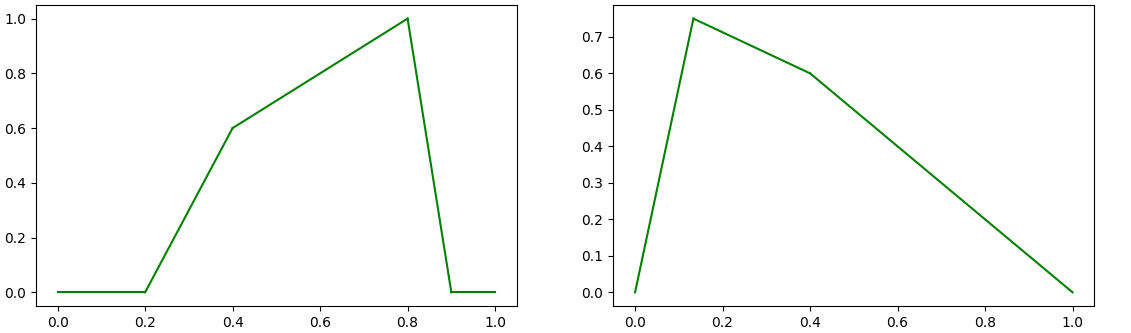
\includegraphics[width=\textwidth]{figures/example3.png}
\caption{Đồ thị của tập mờ $A$ và hàm $f$}
\label{fig:4}
\end{figure}

\begin{figure}[H]
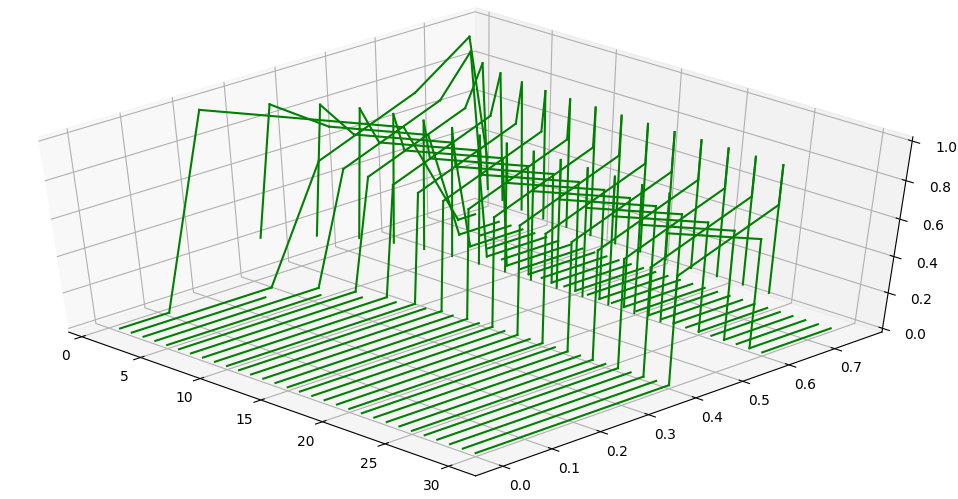
\includegraphics[width=\textwidth]{figures/example3_3d.png}
\caption{30 giá trị đầu tiên của quỹ đạo}
\label{fig:5}
\end{figure}

\begin{figure}[H]
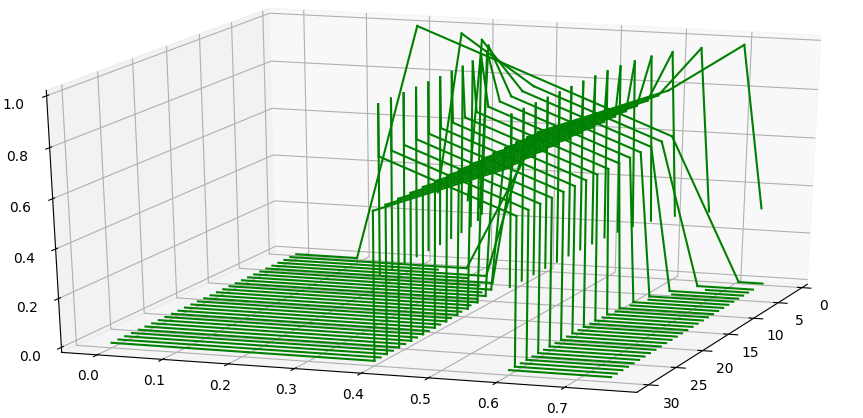
\includegraphics[width=\textwidth]{figures/example3_3d_2.png}
\caption{30 giá trị đầu tiên của quỹ đạo, một góc nhìn khác}
\label{fig:6}
\end{figure}

\noindent \textbf{Ví dụ 4}: Trong ví dụ này ta xem xét đến ánh 
xạ piecewise linear liên tục f và tập mờ piecewise linear 
liên tục A được mô tả trong hình \ref{fig:7}. Ta lại thấy 
rằng vòng lặp thứ 2, tập A trở thành hàm gián đoạn.
Và tương tự hình \ref{fig:8} là 20 bước lặp đầu tiên. 

\begin{figure}[H]
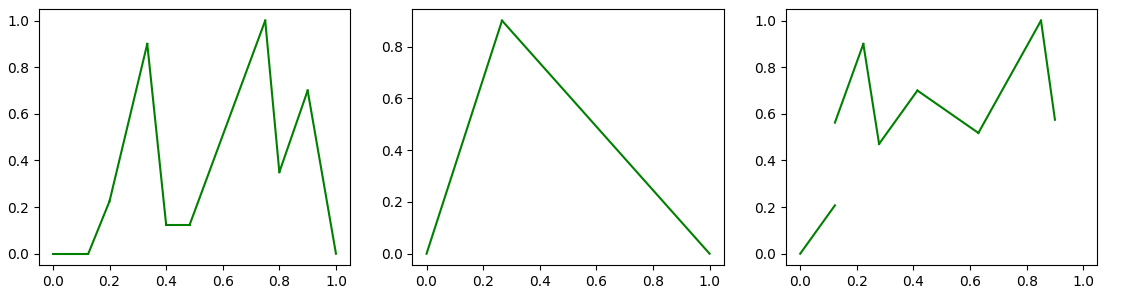
\includegraphics[width=\textwidth]{figures/example4.png}
\caption{Đồ thị của tập mờ $A$, hàm $f$ và $z_f^2(A)$}
\label{fig:7}
\end{figure}

\begin{figure}[H]
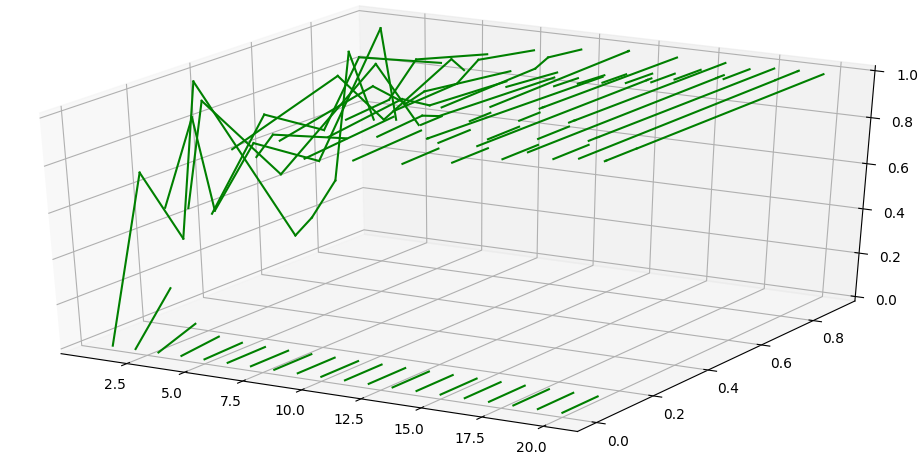
\includegraphics[width=\textwidth]{figures/example4_3d.png}
\caption{20 giá trị đầu tiên của quỹ đạo}
\label{fig:8}
\end{figure}

\subsection{Độ phức tạp thuật toán}

\begin{table}[H]
    
\caption{Độ phức tạp thuật toán theo $ms$}
\begin{center}
\begin{tabular}{|c|c|c|c|}
\hline
Số vòng lặp & 10000 & 100000 &  1000000 \\ 
\hline
\textbf{Ví dụ 2} & 19.0 & 162.5 & 1551.7 \\
\textbf{Ví dụ 3} & 33.2 & 319.0 & 3222.1 \\
\textbf{Ví dụ 4} & 15.2 & 151.0 & 1533.1 \\
\hline
\end{tabular}
\end{center}

\end{table}
Biên dịch trên laptop Intel(R) Core(TM) i3-3217U CPU @ 1.80GHz sử dụng
ngôn ngữ lập trình Rust.

\end{document}
